\documentclass[12pt]{article}
 
\usepackage{afterpage,amssymb,amsmath,amsfonts,eurosym,geometry,
ulem,graphicx,caption,subcaption,color,setspace,sectsty,comment,fnpct,caption,natbib,array,hyperref,float,pdfpages,fancyhdr,pdflscape,amsmath,mathtools,fancyvrb}
\usepackage{xurl}
\usepackage[dvipsnames]{xcolor}
\usepackage[bottom]{footmisc}
\usepackage{booktabs}
\usepackage{pdflscape}
\usepackage{afterpage}
\usepackage{setspace}
\usepackage{longtable}
\usepackage{array}
\usepackage{color}
	\definecolor{maroon}{RGB}{128,0,0}
	\definecolor{navy}{RGB}{0,0,165}
	\definecolor{lb}{RGB}{150,165,190}
    \definecolor{dg}{RGB}{15,92,18}
    \definecolor{purple}{RGB}{145,40,190}
\usepackage{hyperref}
\hypersetup{
     colorlinks = true,
     citecolor = navy,
     linkcolor = navy,
     urlcolor=navy
}

\fancypagestyle{appstyle}{
 \fancyhf{}
 \fancyfoot[C]{\thepage}
 \fancyhead[C]{\textit{Online Appendix}}
}
  
\normalem
\newcommand{\source}[1]{\\ \raggedright {#1}}
\geometry{left=1.0in,right=1.0in,top=1.0in,bottom=1.0in}
 
\newtheorem{theorem}{Theorem}
\newtheorem{acknowledgement}[theorem]{Acknowledgement}
\newtheorem{algorithm}[theorem]{Algorithm}
\newtheorem{axiom}[theorem]{Axiom}
\newtheorem{case}[theorem]{Case}
\newtheorem{claim}[theorem]{Claim}
\newtheorem{conclusion}[theorem]{Conclusion}
\newtheorem{condition}[theorem]{Condition}
\newtheorem{conjecture}[theorem]{Conjecture}
\newtheorem{corollary}[theorem]{Corollary}
\newtheorem{criterion}[theorem]{Criterion}
\newtheorem{definition}[theorem]{Definition}
\newtheorem{example}[theorem]{Example}
\newtheorem{exercise}[theorem]{Exercise}
\newtheorem{lemma}[theorem]{Lemma}
\newtheorem{notation}[theorem]{Notation}
\newtheorem{problem}[theorem]{Problem}
\newtheorem{proposition}[theorem]{Proposition}
\newtheorem{remark}[theorem]{Remark}
\newtheorem{solution}[theorem]{Solution}
\newtheorem{summary}[theorem]{Summary}
\newenvironment{proof}[1][Proof]{\noindent\textbf{#1.} }{\ \rule{0.5em}{0.5em}}

\usepackage[font={large,sc}]{caption}
\usepackage[sc]{mathpazo}
\usepackage[T1]{fontenc}
\VerbatimFootnotes 

\setlength{\tabcolsep}{8pt} % Default value: 6pt
\renewcommand{\arraystretch}{1.5} 
%\newcolumntype{G}{@{\extracolsep{12pt}}c@{\extracolsep{12pt}}}%

\title{QFM Exploration Notes}
\author{}
\date{\today}

\def\cei^#1_#2{\lower\fontdimen17\textfont2\vbox{%
   \baselineskip=\fontdimen17\textfont2 \advance\baselineskip by\fontdimen14\textfont2
   \halign{\hfil$\scriptstyle##$\hfil\cr#1\cr#2\cr}%
}}

\newcommand{\N}{\mathbb{N}}
\newcommand{\Z}{\mathbb{Z}}
\newcommand{\Ztilde}{\mathbf{\Tilde{Z}}}
\newcommand{\E}{\mathbb{E}}

\DeclareMathOperator*{\argmax}{\text{arg} \max}
\DeclareMathOperator*{\argmin}{\text{arg} \min}

\begin{document}

\newgeometry{left=1.0in,right=1.0in,top=1.0in,bottom=1.0in}
\maketitle

\section{Location-Scale Model Notes}

I consider the following DGP:

\begin{equation*}
	y_{it} = \alpha_i\beta_t + \eta_i\gamma_te_{it}
\end{equation*}

\noindent We require that $\eta_t\gamma_t > 0$, so we will draw them from the $\chi^2$ distribution. All together we have:

\[
	\alpha_i \sim \mathcal{N}(0, 1); \quad \beta_t \sim \mathcal{N}(0, 1); \quad \eta_i \sim \chi^2(1); \quad \gamma_t \sim \chi^2(1); \quad e_{it} \sim \mathcal{N}(0,1)
\]

In general, we let $F$ be the cdf of $e_{it}$. Then the conditional quantile function is:

%
\begin{equation*}
	Q_{\tau }(y_{it}|\alpha_i, \beta_t, \eta_i\gamma_t)=\alpha_i\beta_t + \eta_i\gamma_t F^{-1}(\tau)= \alpha_i\beta_t + \eta_i\gamma_t Q(\tau)
\end{equation*}
%

We call the estimates of this conditional quantile function from the QPC algorithm $\hat{\alpha}, \hat{\beta}, \hat{\eta}, \hat{\gamma}$. If the algorithm converges to the true values (as captured by the common component), we would expect that the estimated factors span the same space as the true ones. Because the rotation of the factors is not identified, we need to measure this in a way that is invariant to rotation. To do so, we consider the $R^2$ of the following regressions:

\begin{equation*}
	\beta = a + b_1\hat{\beta} + b_2\hat{\gamma}; \quad \gamma = c + d_1\hat{\gamma} + d_2\hat{\gamma};
\end{equation*}

If the algorithm is converging properly, we would expect high values of $R^2$ in each of these regressions.

Note that under this DGP, beacuse $e_it$ is $\mathcal{N}(0, 1)$ we have that at the median $(\tau = 0.50)$ there will only be one factor.  

For now, I will consider the errors-in-variables rotation, where with $k_{\tau}$ factors, the factor loadings are restricted such that $\Lambda = \left[I_{k_{\tau}} \space \Lambda_2\right]^{\prime}$. This is the most simple computationally, though there are others I could consider from \citet{BaiNg2013}.

For now, I want to see how this DGP behaves and wether we can do any estimation consistently. My target is to replicate table 2 from \citet{Sagner2019}, shown in Figure \ref{fig:sagner_t2}.

\afterpage{%
    \clearpage% Flush earlier floats (otherwise order might not be correct)
    \thispagestyle{empty}% empty page style (?)
    \begin{landscape}% Landscape page
        \begin{figure}[ht]
            \centering
            \caption{}
            \label{fig:sagner_t2}
            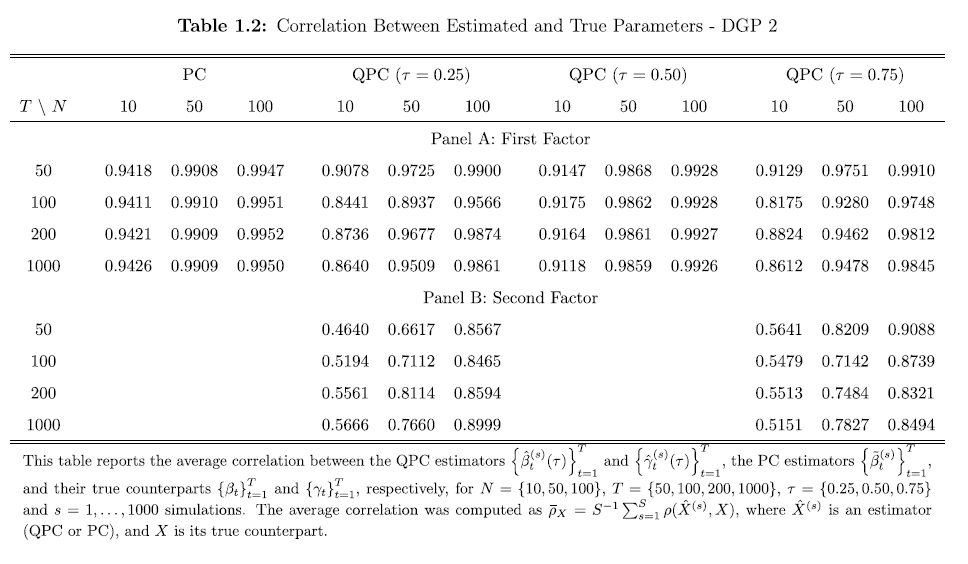
\includegraphics[width=0.9\linewidth]{../out/sagner_t2.png}
        \end{figure}
    \end{landscape}
    \clearpage% Flush page
}

I will not report PC estimates. In addition to the mean $R^2$ values for both the first and second factor, I will include the proportion of simulations where the process took a long time to converge ($> 100$ iterations), where it didn't converge at all (not converged at $1000$ iterations), the proportion of simulations where the $R^2$ for the second factor is $> 0.5$, and the proportion of simulations where the $R^2$ of the first factor is $< 0.9$. For small $N$ and $T$ this last value may be sizable, but for larger $N$ and $T$ a large value of this proportion is concerning as it implies that the first factor is not being estimated consistently.

I want to first check that my estimation procedure is working correctly. To do so, I will consider 2 simple DGPs:

\begin{align}
    y_{it} &= \alpha_i\beta_t + e_{it} \label{eq:dgp1} \\ 
    y_{it} &= \alpha_i\beta_t + \eta_i\gamma_t + e_{it} \label{eq:dgp2}
\end{align}

\noindent These DGPs are simple location models, and so we should expect a good fit for both the one factor case (Equation \ref{eq:dgp1}) and the two factor case (Equation \ref{eq:dgp2}). Results of a small simulation study are reported in. 

\clearpage

Now that the simulation is behaving as anticipated, I will explore the question of initial values. For this study, I consider the following DGP:

\begin{equation}
    y_{it} = \alpha_i\beta_t + \eta_i\gamma_te_{it} \label{eq:dgp3}
\end{equation}

Where $\eta_i, \gamma_t \sim \chi^2_1$ to satisfy $\eta_i\gamma_t > 0$. I fit a QFM using the same procedure as before, but with a change in the initialization step. Instead of beginning with PCA to guess the initial values, I add noise from a $\mathcal{N}(0, 1)$ to the initial PCA estimate. This is then rotated according to the errors-in-variables rotation I have used previously. The model is fit from these new initial values, and some interesting patterns appear. Consider the examples in tables \ref{tab:ivdiff_results_badsf}, \ref{tab:ivdiff_results_badff}, and \ref{tab:ivdiff_results_goodbf}.

\begin{table}[ht]
    \begin{center}
        \caption{QFM Fits With Different Noise - Bad Second Factor Fit}
        \label{tab:ivdiff_results_badsf}
        \scalebox{0.8}{
            % latex table generated in R 4.3.2 by xtable 1.8-4 package
% Wed Apr  9 12:04:13 2025
\begin{tabular}{ccccc}
   
Noise Seed & First Factor Fit & Second Factor Fit & Iterations & Objective Function Value \\
 \hline
No Noise & 0.9921 & 0.1600 &    14 & 3909.9828 \\ 
  134935 & 0.9912 & 0.7791 &    33 & 3595.2488 \\ 
  363439 & 0.9924 & 0.7245 &    18 & 3645.0155 \\ 
  880628 & 0.9927 & 0.1601 &    24 & 4005.6856 \\ 
  252318 & 0.9954 & 0.7844 &    84 & 3677.4222 \\ 
  344982 & 0.9965 & 0.7391 &    16 & 3591.6591 \\ 
  702677 & 0.9920 & 0.8051 &    54 & 3555.9745 \\ 
  116075 & 0.9910 & 0.1600 &    19 & 3915.6519 \\ 
  100298 & 0.9934 & 0.7755 &    25 & 3667.7547 \\ 
  178700 & 0.9943 & 0.1599 &    28 & 3940.8150 \\ 
  310893 & 0.9903 & 0.7956 &    28 & 3564.4116 \\ 
  True & 0.9950 & 0.8008 &    47 & 3525.9113 \\ 
  \end{tabular}

        }
    \end{center}
    {\small \begin{singlespace} \textbf{Notes:} This table reports the $R^2$ value for a regression each of the true factors on the estimated factors, as well as the value of the objective function evaluated at the estimate. Each observation is a different seed for random noise added to initial values generated by PCA.\end{singlespace}}
\end{table}

\begin{table}[ht]
    \begin{center}
        \caption{QFM Fits With Different Noise - Poor PCA Fit}
        \label{tab:ivdiff_results_badff}
        \scalebox{0.8}{
            % latex table generated in R 4.3.2 by xtable 1.8-4 package
% Wed Apr  9 12:01:46 2025
\begin{tabular}{ccccc}
   
Noise Seed & First Factor Fit & Second Factor Fit & Iterations & Objective Function Value \\
 \hline
No Noise & 0.0119 & 0.0639 &     3 & 4548.2392 \\ 
  32851 & 0.9983 & 0.4868 &    91 & 2921.2252 \\ 
  305155 & 0.9985 & 0.1999 &    28 & 3004.2602 \\ 
  530302 & 0.9979 & 0.0911 &    26 & 3056.5396 \\ 
  53515 & 0.9965 & 0.4573 &    21 & 2967.1183 \\ 
  965115 & 0.9975 & 0.0176 &   100 & 3185.0630 \\ 
  201177 & 0.0703 & 0.3880 &    95 & 4157.0256 \\ 
  380261 & 0.9975 & 0.0422 &    11 & 3015.5472 \\ 
  406115 & 0.9982 & 0.0828 &   100 & 3128.7703 \\ 
  445781 & 0.9974 & 0.3452 &    15 & 2956.7660 \\ 
  912360 & 0.9981 & 0.3322 &    72 & 2969.2764 \\ 
  True & 0.9971 & 0.5003 &     7 & 2901.3943 \\ 
  \end{tabular}

        }
    \end{center}
    {\small \begin{singlespace} \textbf{Notes:} This table reports the $R^2$ value for a regression each of the true factors on the estimated factors, as well as the value of the objective function evaluated at the estimate. Each observation is a different seed for random noise added to initial values generated by PCA.\end{singlespace}}
\end{table}

\begin{table}[ht]
    \begin{center}
        \caption{QFM Fits With Different Noise - Good PCA Fit}
        \label{tab:ivdiff_results_goodbf}
        \scalebox{0.8}{
            % latex table generated in R 4.3.2 by xtable 1.8-4 package
% Wed Apr  9 11:59:25 2025
\begin{tabular}{ccccc}
   
Noise Seed & First Factor Fit & Second Factor Fit & Iterations & Objective Function Value \\
 \hline
No Noise & 0.9969 & 0.8077 &    68 & 3119.1333 \\ 
  688017 & 0.9968 & 0.8088 &    48 & 3112.0576 \\ 
  7268 & 0.9971 & 0.7998 &    20 & 3155.9562 \\ 
  934064 & 0.9969 & 0.8006 &    25 & 3164.4899 \\ 
  343860 & 0.9974 & 0.7982 &    18 & 3141.5936 \\ 
  798375 & 0.9965 & 0.7849 &    19 & 3050.5442 \\ 
  631366 & 0.9967 & 0.7847 &    71 & 3257.3209 \\ 
  124501 & 0.9957 & 0.7886 &    38 & 3184.5473 \\ 
  163844 & 0.9959 & 0.7902 &    51 & 3116.7062 \\ 
  673964 & 0.9975 & 0.7865 &    45 & 3170.8194 \\ 
  272234 & 0.9973 & 0.7840 &    19 & 3144.6454 \\ 
  True & 0.9992 & 0.8096 &    10 & 2989.2456 \\ 
  \end{tabular}

        }
    \end{center}
    {\small \begin{singlespace} \textbf{Notes:} This table reports the $R^2$ value for a regression each of the true factors on the estimated factors, as well as the value of the objective function evaluated at the estimate. Each observation is a different seed for random noise added to initial values generated by PCA.\end{singlespace}}
\end{table}

In table \ref{tab:ivdiff_results_badsf}, the fit based on the PCA starting values is quite poor for the second factor. Using different starting values, I am able to get a better fit for the second factor which is mirrored with a large decrease in the value of the objective function. Adding noise can also make the fit worse in terms of objective function value. 

In table \ref{tab:ivdiff_results_badff}, the fit based on the PCA starting values is quite poor for both factors. Using different starting values, the fit is improved dramatically with the first factor being fit well and the second factor being fit decently. 

In table \ref{tab:ivdiff_results_goodbf}, the fit based on the PCA starting values is very good. However, different starting values can produce a lover value of the objective function. 

\clearpage

Next, I consider starting estimation with the true factor levels and loadings. In each of the 3 examples above, using the true levels and loadings improves the fit and lowers the objective function value. I think this can be thought of as the ideal scenario, at least for the angle from which I am approaching the problem. The trouble we have with PCA is that it is based on the mean, and so is uninformative of the true value of the second factor because at the median, the second factor doesn't contribute. We want the initial value to be close to the true value so that we are close to the global optimum in the objective function. This is then a benchmark against which methods can be compared.

\pagebreak \newpage
\singlespacing
%\setlength \bibsep{0pt}
\bibliographystyle{harvard}
%\bibliographystyle{humannat}
\bibliography{literature}

\end{document}


























